\section{Results}
    \subsection{Classification}
        % Table with the one best accuracy score from the two methods
        % Figure with analysis of regularization parameters and learning rates
        
        Following are some results from the neural network classification project. Figure \ref{fig:ANNREG1} illustrates the accuracy scores for network $N3$:
        \begin{figure}
            \centering
            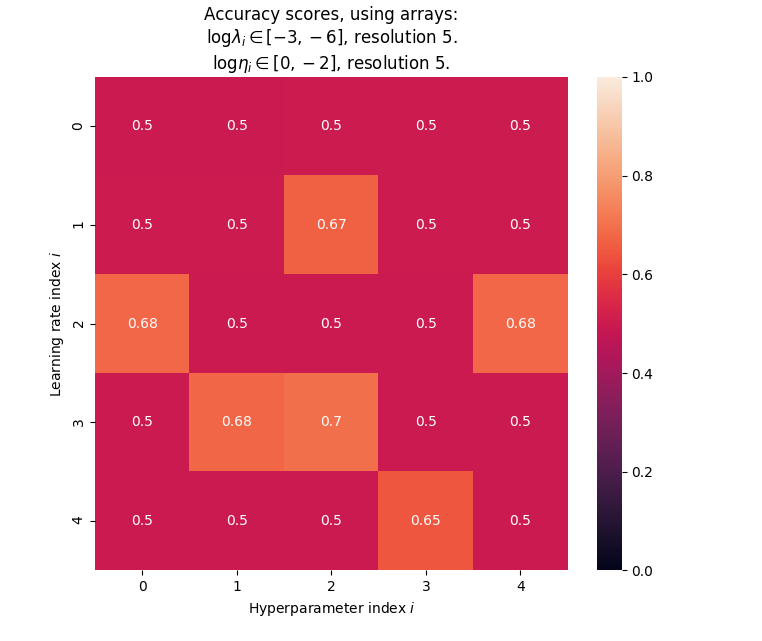
\includegraphics[width=0.4\textwidth]{figures/Ngrid3_acc.png}
            \caption{Grid search with label $N3$ results. This figure illustrates the accuracy scores for several neural networks with various hyperparameters $\lambda$ and learning rates $\eta$. The range and resolutions of the parameters are in the title, while the indices of the axes range from largest to smallest.}
            \label{fig:ANNREG1}
        \end{figure}
        Figure \ref{fig:ANNREG2} illustrates the area under the cumulative gain curve for network $N3$:
        \begin{figure}
            \centering
            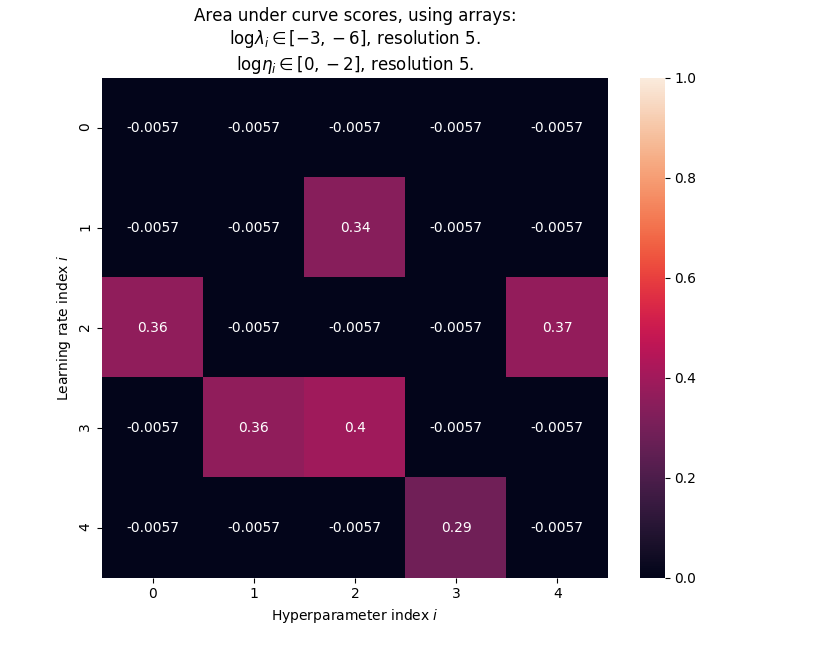
\includegraphics[width=0.4\textwidth]{figures/Ngrid3_auc.png}
            \caption{Grid search with label $N3$ results. This figure illustrates the area under the cumulative gain curve for several neural networks with various hyperparameters $\lambda$ and learning rates $\eta$. The range and resolutions of the parameters are in the title, while the indices of the axes range from largest to smallest.}
            \label{fig:ANNREG2}
        \end{figure}
        Figure \ref{fig:ANNREG3} illustrates the $F1$ scores for network $N3$:
        \begin{figure}
            \centering
            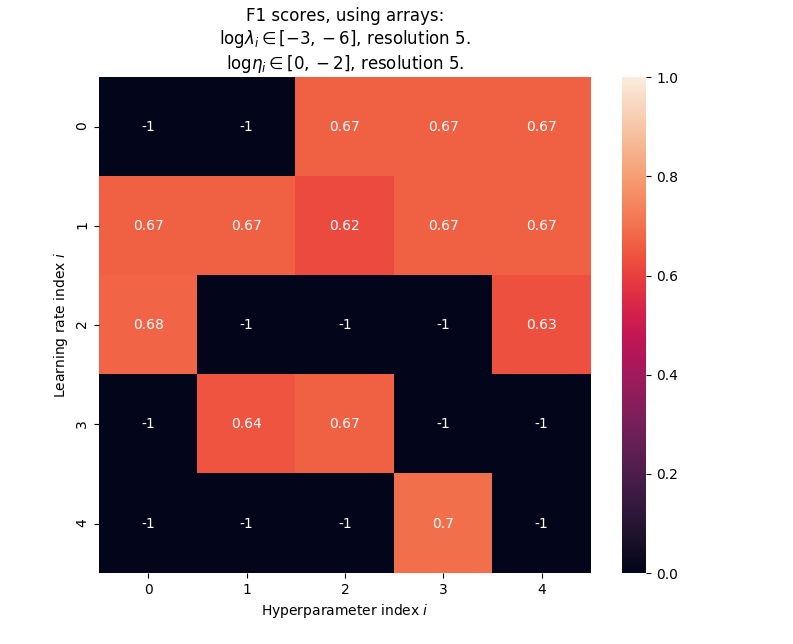
\includegraphics[width=0.4\textwidth]{figures/Ngrid3_F1.png}
            \caption{Grid search with label $N3$ results. This figure illustrates the $F1$ for several neural networks with various hyperparameters $\lambda$ and learning rates $\eta$. The range and resolutions of the parameters are in the title, while the indices of the axes range from largest to smallest.}
            \label{fig:ANNREG3}
        \end{figure}
        
        
    \subsection{Regression}
        Following is a table from project 1, listing the precision of three regression schemes applied to Franke's function:
        \begin{table}[H]
            \centering
            \caption{Table listing the final results and comparisons of the regressional methods applied to Franke's function with $n=10,000$ data points.}
            \begin{tabular}[t]{l@{\hskip 0.3in}c@{\hskip 0.3in}c@{\hskip 0.2in}c}
                \toprule
                Scheme & MSE minimum & $p_{deg}$ & $\log(\lambda)$ \\
                \midrule
                OLS & 0.2493 & 8 & $-$\\
                Ridge & 0.2489 & 11 & -9\\
                Lasso & 0.2524 & 8 & -12\\
                \bottomrule
            \end{tabular}
            \label{tab:conclusion_table_Frankes}
        \end{table}
        
        
        \begin{figure}
            \centering
            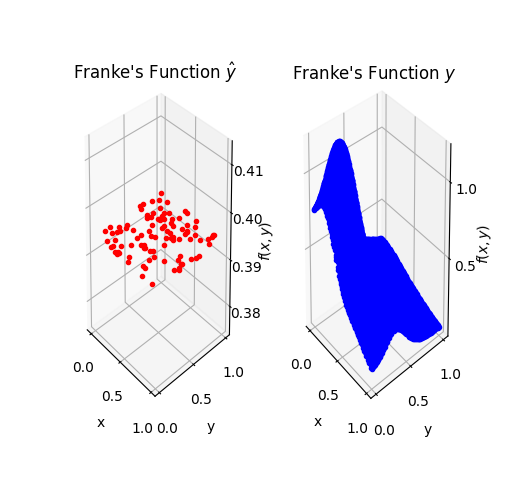
\includegraphics[width=0.4\textwidth]{figures/regression_NNW.png}
            \caption{The ANN regression on Franke's function. With $MSE=4.08$.}
            \label{fig:ANNREG}
        \end{figure}
        
        
        % Table with the least MSE from the two methods
        % (Figure with analysis of regularization parameters and learning rates): this is not specifically asked for in the problem set, it wants: a discussion of reg. params./learning rates